
%(BEGIN_QUESTION)
% Copyright 2006, Tony R. Kuphaldt, released under the Creative Commons Attribution License (v 1.0)
% This means you may do almost anything with this work of mine, so long as you give me proper credit

Examine the loop diagram for a laboratory gasoline flow control system:

$$\includegraphics[width=15.5cm]{i00711x01.eps}$$

This system used to work just fine, but now it has a problem: the controller registers zero flow, and its output signal (to the valve) is saturated at 100\% (wide open) as though it were trying to ``ask'' the valve for more flow.  Your first diagnostic step is to check to see if there actually is gasoline flow through the flowmeter and valve by looking at the rotameter.  You see that the rotameter is ``pegged'' at over 2 GPH of flow.

Identify two possible faults in this system that could account for the controller's condition and the rotameter's indication:

\begin{itemize}
\item{} Possible fault:
\vskip 10pt
\item{} Possible fault:
\end{itemize}

\underbar{file i00711}
%(END_QUESTION)





%(BEGIN_ANSWER)

5 points for each correct answer:

\begin{itemize}
\item{} Possible fault: {\it Turbine jammed so it cannot rotate}
\item{} Possible fault: {\it 4-20 mA signal wires from transmitter failed open}
\end{itemize}

%(END_ANSWER)





%(BEGIN_NOTES)

{\bf This question is intended for exams only and not worksheets!}.

%(END_NOTES)


